\documentclass{article}
\usepackage[utf8]{inputenc}
\usepackage[T1]{fontenc}
\usepackage[french]{babel}
\usepackage{hyperref}
\usepackage{graphicx}
\usepackage{algorithm}
\usepackage{algpseudocode}
\hypersetup{
    colorlinks,
    citecolor=black,
    filecolor=black,
    linkcolor=blue,
    urlcolor=blue,
}
\title{Analyse des algorithmes de tris}
\author{Fouché Stanislas \\ Hill Tom \\ Leveziel Damien \\ Boulay Dimitri}
\date{Mars 2023}

\begin{document}

\maketitle
\newpage
\tableofcontents
\newpage
\section{Objectifs du projet}

\subsection{Problématique du projet}
Un algorithme de tri est un algorithme qui va permettre d'organiser une collection d'objets selon une relation. Il existe une multitude d'algorithmes de tri, au fonctionnement et à l'efficacité différentes. La plupart de ces algorithmes sont basés sur de la comparaison entre des éléments. Cependant, les éléments choisis pour ces comparaisons sont la différence fondamentale entre ces algorithmes. Certains de ces algorithmes sont peu efficaces, et la plupart dépendent de la structure des éléments à comparer. Nous nous demandons comment varie l'efficacité des ces algorithmes selon le type de tri en fonction du désordre des données. Au delà de comparer les temps d'exécution nous souhaitons aussi visualiser le nombre de comparaisons et l'accès aux données. Pour ce faire nous devons implémenter un certain nombre de ces algorithmes et les comparer sur des tableaux de données similaires pour constater leur efficacité. 

\subsection{Choix} %pourquoi java, choix des algorithmes
On a choisit d'utiliser java parce qu'il était plus simple d'utiliser les adresses des tableaux en java, étant donné qu'on y était déjà tous habitués. De plus, la visualisation est plus simple à effectuer qu'en python, surtout si on veut faire une application qui trie des tableaux en boucle. Enfin, faire ce projet en java permettait d'approfondir notre connaissance au langage objet, ce qui faisait de java le langage qu'on préférait utiliser

\subsection{Description des point clés du projet}
Les points clés du projet sont dans un premier temps l'implémentation du générateur de tableau avec plusieurs de types de mélanges. Après avoir généré un tableau, le choix des algorithmes de tri ; il a fallu choisir des algorithmes pertinents à comparer avec des complexités différentes. Il a ensuite fallu implémenter ces algorithmes. Nous avons créé une interface graphique permettant de visualiser le fonctionnement de ces algorithmes en direct après les avoir fait. Et enfin, nous avons créé de quoi tester ces algorithmes et voir leur différences.

\section{Fonctionnalités implémentées}

\subsection{Répartition du travail}

Pour commencer, chacun de nous a implémenté de 3 à 4 algorithmes de tri.
Ensuite il fallait disperser les taches restantes : 
\begin{itemize}
    \item Génération de tableau aléatoires : Damien et Dimitri 
    \item Interface Graphique : Dimitri et Tom
    \item Mise en forme des résultats expérimentaux : Damien et Tom 
    \item Tests et la mise en place d'un ant : Stanislas
\end{itemize}

\section{Éléments techniques}

\subsection{Description du générateur de données}
Il à été décidé de choisir comme données des tableaux d'entiers, ce sont des données simples et facilement manipulâmes. Le générateur va créer des tableaux de la taille désirée, avec des entiers allant de 1 à n (n étant la taille désirée). Ensuite selon le type de mélange choisi et l'entropie, le générateur va mélanger ce tableau. Il existe différents types de mélanges : 
\begin{itemize}
    \item Le mélange simple : Le générateur va faire X inversions aléatoires dans le tableau. (Avec X l'entropie)
    \item Le reverse : Le générateur va inverser le tableau. Généralement ce mélange permet de montrer la pire complexité des algorithmes.
    \item La fin mélangée : Le générateur va faire X inversions dans les 25 derniers \% du tableau, le reste est trié dans l'ordre.
\end{itemize}
\subsection{Description des algorithmes}
Pour le bien de ce projet nous avons dû implémenter une dizaine d'algorithmes de tri aux complexités et au fonctionnement différents.

% une \subsubsection{} par algo, où on explique le principe rapidement
\subsubsection{BubbleSort}
    \label{BubbleSort}
\footnotesize 
\noindent
Complexité :  $ n^2$
\\
\normalsize
Cet algorithme est un algorithme basique qui va seulement inverser deux éléments si ils ne sont pas dans le bon ordre. Il est en théorie inefficace sur des grands tableaux de données.
\subsubsection{InsertionSort}
    \label{InsertionSort}
\footnotesize 
\noindent
Complexité :  $ n^2$
\\
\normalsize
Le tri par insertion est un tri basique. Il fonctionne de la manière suivante. L'algorithme va créer un tableau secondaire où à chaque passage dans le tableaux de données, il va la placer à son emplacement dans le tableau secondaire.
\subsubsection{BogoSort}
    \label{BogoSort}
\footnotesize 
\noindent
Complexité :  $ (n+1)!$
\\
\normalsize
Cette algorithme est l'algorithme de tri le plus inefficace, il consiste seulement à mélanger aléatoirement le tableau à chaque itération et vérifier si les données sont triées. Il est utilisé généralement comme comparaison aux autres algorithmes de tri. Nous l'avions implémenté à la base pour tester notre génération de tableaux.
\subsubsection{CombSort}
    \label{combSort}
\footnotesize 
\noindent
Complexité :  $ n^2$
\\
\normalsize
Le CombSort (ou tri à peigne) est une amélioration de l'algorithme BubbleSort \ref{BubbleSort}. Au lieu de prendre chaque élément adjacent un par un, il prendra les éléments avec un espacement différent à chaque itération. L'espacement initial est égal à la taille de la liste, puis il est divisé par 1,3 à chaque itération. Le choix de 1,3 n'est pas anodin, il à été trouvé empiriquement sur beaucoup de listes pour savoir quelle valeur est optimale.
\subsubsection{GnomeSort}
    \label{GnomeSort}
\footnotesize 
\noindent
Complexité :  $ n^2$
\\
\normalsize
Le Gnome Sort est une variation du Tri par insertion (\ref{InsertionSort}) dont la principale différente est le fait qu'il ne passe pas par une deuxième tableau, il consiste en un parcours des données, et à chaque fois l'algorithme va prendre la valeur choisie et la suivante. Si la valeur suivante est inférieure il va échanger ces deux valeurs ensuite retourner à la valeur précédente du tableau. Si la valeur est suivante est supérieure, il va avancer jusqu'à la valeur suivante. Jusqu'à la fin du tableau.
\subsubsection{QuickSort}
    \label{quickSort}
\footnotesize 
\noindent
Complexité :  $ n\log n$
\\
\normalsize
Le Quick Sort est l'algorithme considéré comme le plus efficace pour trier un tableau. Il prend une valeur choisie, soit au hasard, à droite, à gauche ou au centre du tableau, et met cette valeur à sa place, avec toutes les autres valeurs inférieures à sa gauche, et supérieure à droite. Après avoir placé la valeur, on peut aller sur le tableau de gauche et de droite récursivement et faire la même chose pour faire des partitions qui ne sont pas loin d'être terminées, et qui auront une complexité de moins en moins grande.
\subsubsection{PancakeSort}
    \label{pancakeSort}
\footnotesize 
\noindent
Complexité :  $ n^2$
\\
\normalsize
    Le pancake sort est un algorithme très peu , mais est un algorithme visuel et facile à comprendre. Pour ce faire, on prend la valeur la plus petite entre la partie du tableau non triée et la partie triée, puis on la met à la fin en renversant tout le tableau entre cette valeur et la dernière. Cela fait que la plus petite valeur est à la fin, puis on renverse tout le tableau non trié une nouvelle fois pour avoir la valeur nécessaire juste après la partie triée. Puis on incrémente de un la taille du tableau trié, et on recommence.
\subsubsection{HeapSort}
    \label{heapSort}
\footnotesize 
\noindent
Complexité :  $ n\log n$
\\
\normalsize
Le Heap sort est une amélioration du \href{https://www.geeksforgeeks.org/selection-sort/}{Tri par sélection}, mais en utilisant la structure d'un arbre binaire. Nous allons chercher l'élément minimal et le mettre au début. Et répéter jusqu'à la fin de l'exécution.
\subsubsection{Radix}
    \label{Radix}
\footnotesize 
\noindent
Complexité :  $n$
\\
\normalsize
Radix est un tri qui n'utilise pas le principe de comparaison.
Le principe est de compter le nombre d'occurrences de chaque entier, et avec ceci on peut calculer un index pour chaque nombre dans la liste triée et recréer une liste en parcourant notre liste à trier et mettant chaque nombre à l'index calculé pour lui.

Il faut un astuce supplémentaire pour trier, car on ne peut pas faire un tableau d'indices de 2 milliards d'entrées. On faut le tri sur les 8 derniers bits, puis à partir de cette nouvelle liste on prends les 8 prochains bits, et après 4 itérations notre entier est triée.
\subsubsection{ShakerSort}
    \label{ShakerSort}
\footnotesize 
\noindent
Complexité :  $ n^2$
\\
\normalsize
Le Tri shaker est une variante du Tri à Bulles (\ref{BubbleSort}) bidirectionnel, qui va changer de direction à chaque passage le long de la liste à trier. Il est en théorie plus efficace que le tri à bulles car il va permettre de gérer les éléments de faible valeur qui vont rester en fin de liste en remontant lentement.
\subsubsection{ShellSort}
    \label{ShellSort}
\footnotesize 
\noindent
Complexité :  $n^{4/3}$
\\
\normalsize
Le tri de Shell est une amélioration du tri par insertion (\ref{InsertionSort}). Le tri de Shell trie les éléments séparés de \emph{n} positions. L'algorithme diminue la valeur de \emph{n} à chaque itération jusqu'à que \emph{n} soit égal à 1. La valeur de diminution de \emph{n} à été trouvée empiriquement et est 2.3.
\subsubsection{MergeSort}
    \label{MergeSort}
\footnotesize 
\noindent
Complexité :  $ n\log n$
\\
\normalsize
Le tri fusion est un algorithme de tri par comparaison. Il va rassembler deux listes triées en une seule. La caractéristique principal de ce tri est qu'il utilise une zone de mémoire deux fois plus grande que le tableau de base car il doit en créer une copie. 
    
\section{Architecture du projet}

\subsection{Diagrammes des classes}
    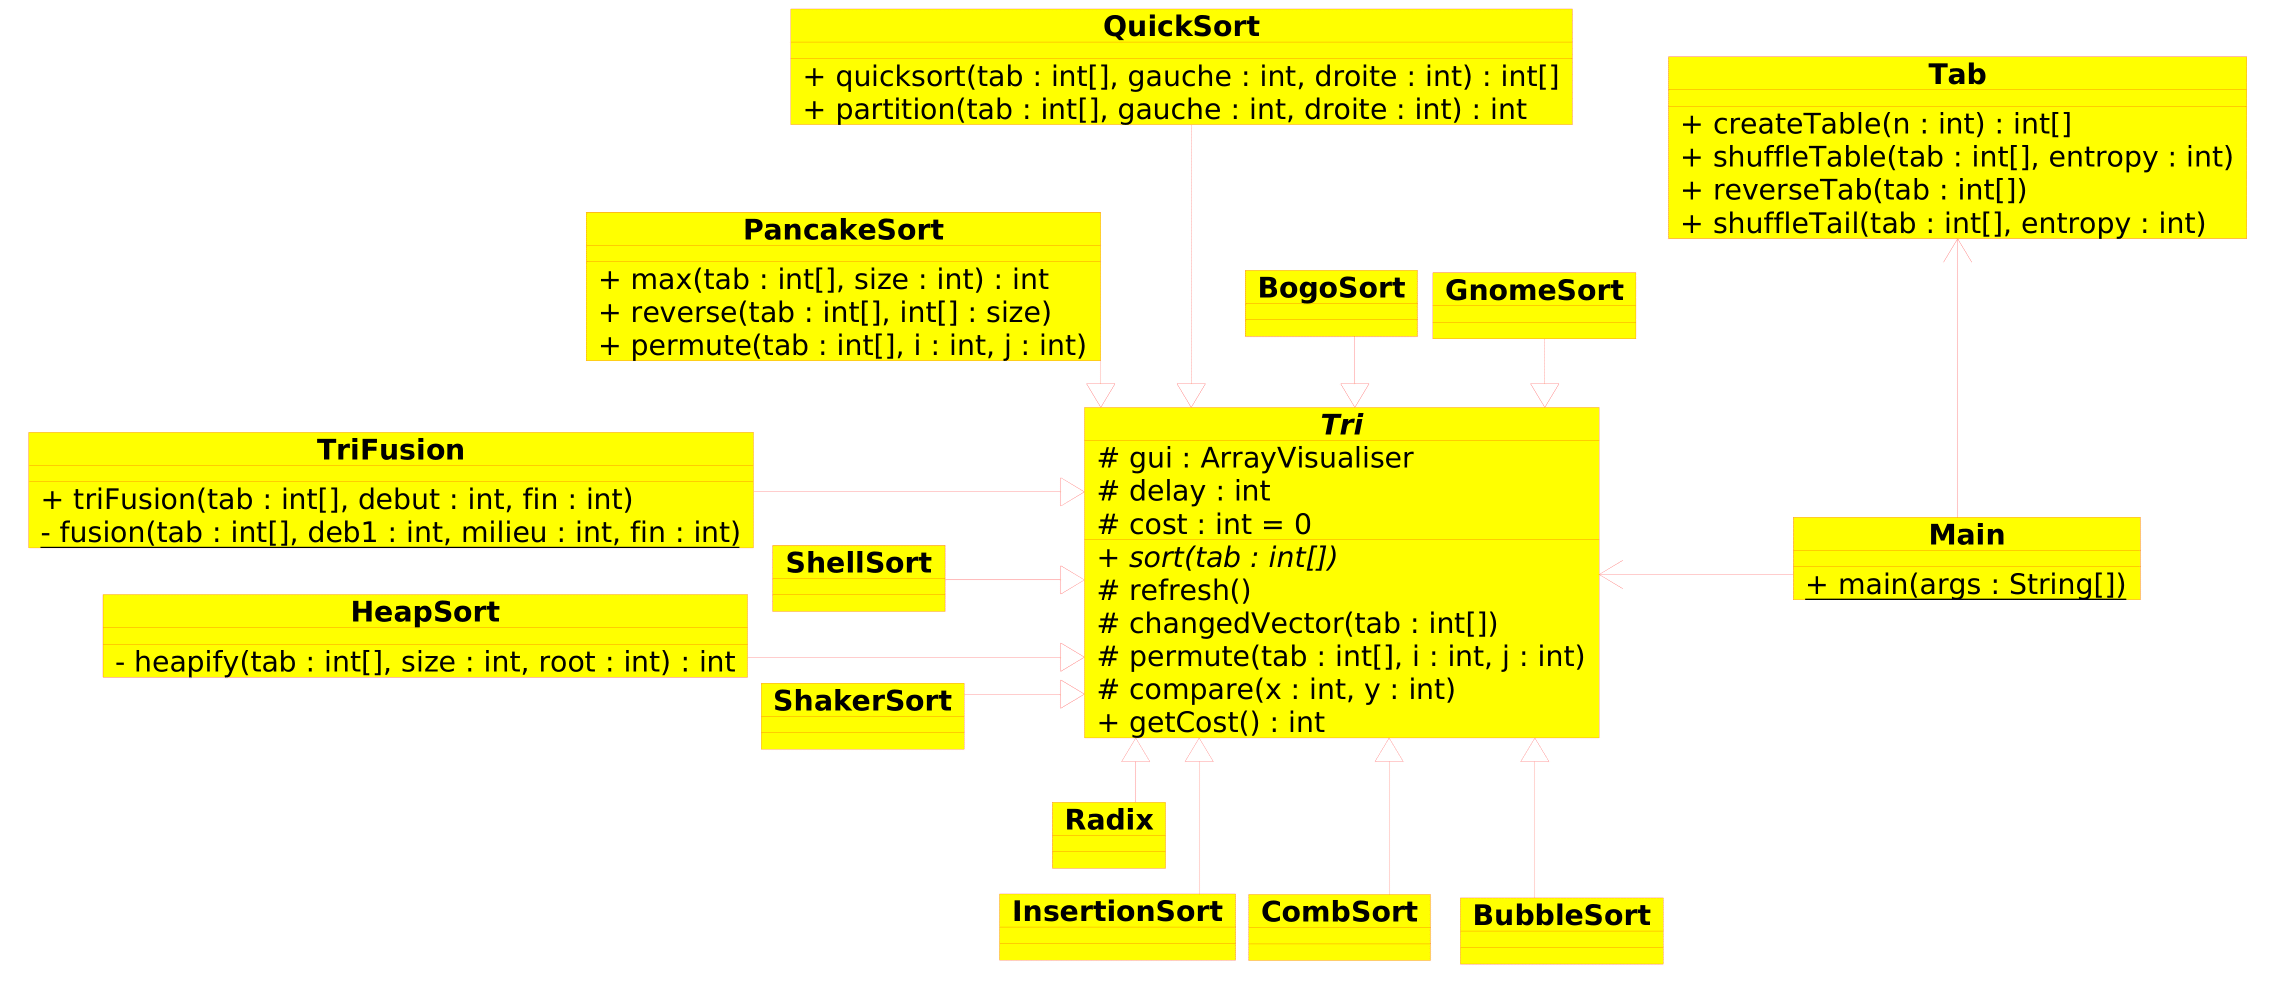
\includegraphics[scale=0.4]{Annexes/DiagramClass-1.png}
    \\La classe Tab créé le tableau, qu'on mélange juste après, que l'on va trier. La classe Main prend alors un Tri, quel qu'il soit, afin de trier ce tableau. Grâce à l'héritage, il est facile d'utiliser n'importe quel algorithme de trie que l'on a.

\subsection{Ant}

On a utilisé un ant pour gérer notre projet : 

\begin{itemize}
    \item \verb|ant compile| : pour simplement compiler l'application
    \item \verb|ant dist| : pour compiler l'application, créer le fichier \verb|jar| et placer ce dernier dans le répertoire \verb|/dist| du projet
    \item \verb|ant run| ou \verb|ant| : pour exécuter l'application
    \item \verb|ant test| : pour exécuter les tests
    \item \verb|ant javadoc| : pour générer la javadoc de l'application
\end{itemize} 

Si le tests unitaires ne fonctionnent pas depuis le ant on peut utiliser éclipse pour voir que nos tests fonctionne. (problème de librairie) 

Les tests cherchent juste à prouver que les algorithmes fonctionnent.

\subsection{Lancement algorithme}

Pour effectuer une simulation d'un des algorithmes, il faut aller dans le fichier src/Main.java et choisir 
les options à lancer : 

\begin{itemize}
    \item taille du tableau 
    \item entropy 
    \item reverse 
    \item choisir l'algorithme ( de préférence mettre sous commentaires les algo non utilisé)
\end{itemize}

il ne reste plus qu'a utilisé la commande : \textbf{ant} ou \textbf{ant run} (run est le lancement par défault) 

\vspace{1cm}

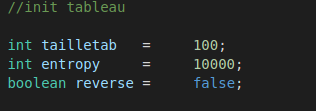
\includegraphics[scale=0.4]{Annexes/init tab.png}
\newline
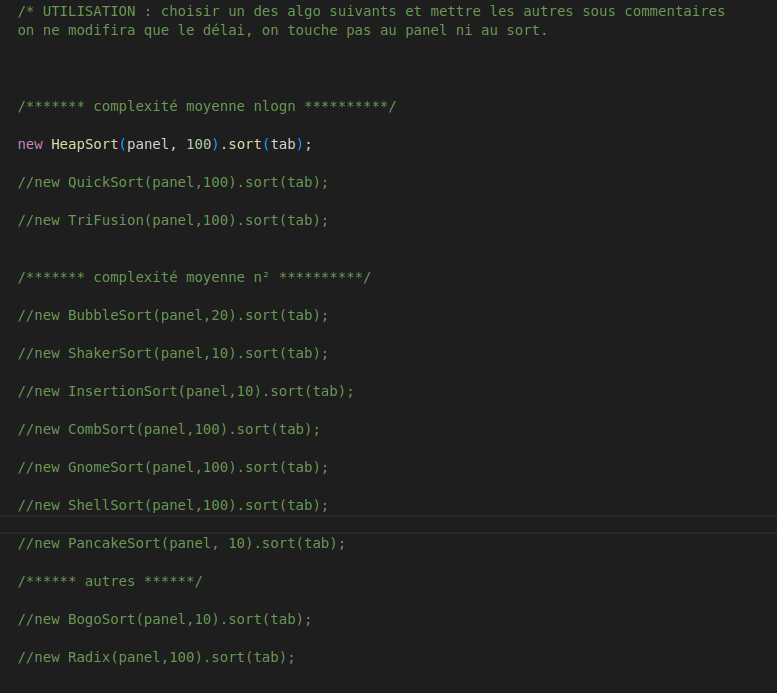
\includegraphics[scale=0.4]{Annexes/choix algo.png}




\section{Expérimentations}

\subsection{Descriptions des cas d'expérimentation}
Pour l'analyse de nos données, nous avons distinguées 4 cas:
\begin{enumerate}
    \item Un tableau trié aléatoirement, avec pour but de voire l'efficacité de l'algorithme sous un contexte couramment rencontré
    \item Un tableau trié avec une très faible entropie, avec pour but de voire si avec peu de corrections à faire l'algorithme savait être plus rapide
    \item Un tableau renversé et ensuite trié avec une faible entropie, avec pour but de voire si l'algorithme savait gérer un cas quasi pire efficacement
    \item Un tableau avec uniquement la fin du tableau trié, avec pour but similaire que la faible entropie, mais pour les algorithmes nlogn qui utilisent souvent le principe de diviser pour régner on peut s'attendre à des différences
\end{enumerate}
\subsection{Résultats expérimentaux}
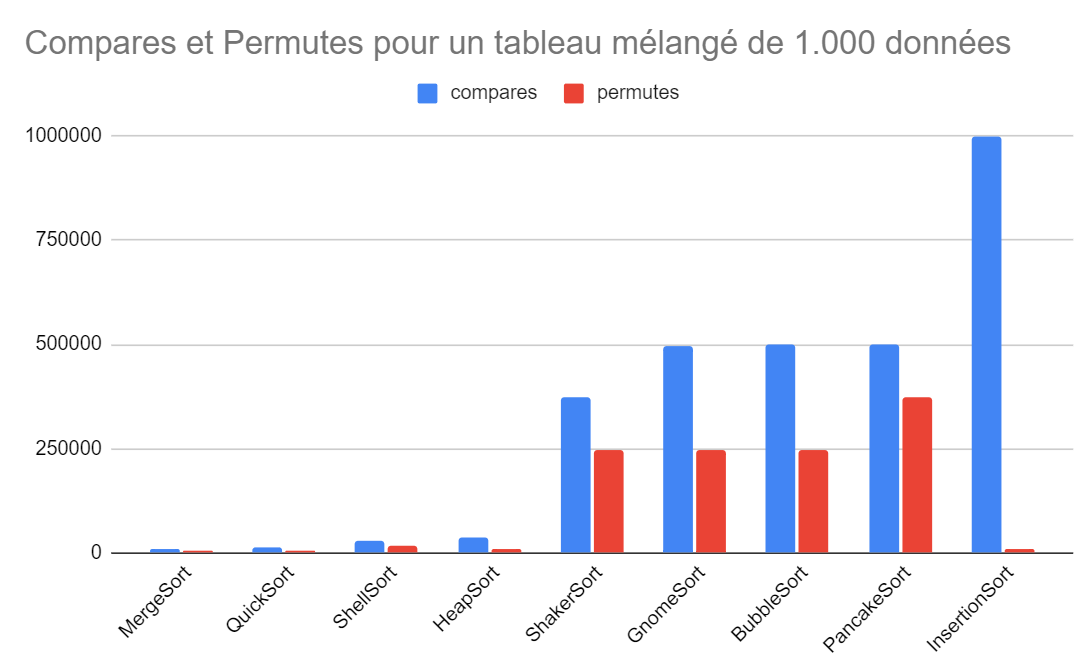
\includegraphics[scale=0.4]{Annexes/GrapheComparePermuteAll.PNG}
\newline
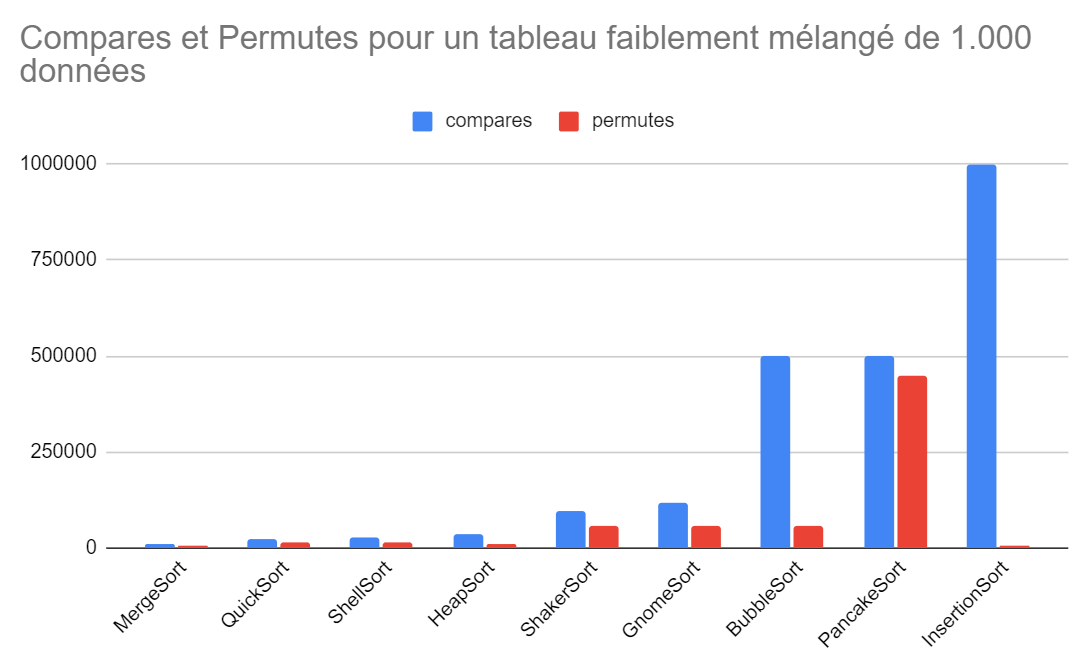
\includegraphics[scale=0.4]{Annexes/GrapheComparePermuteAllFaible.PNG}
\newline
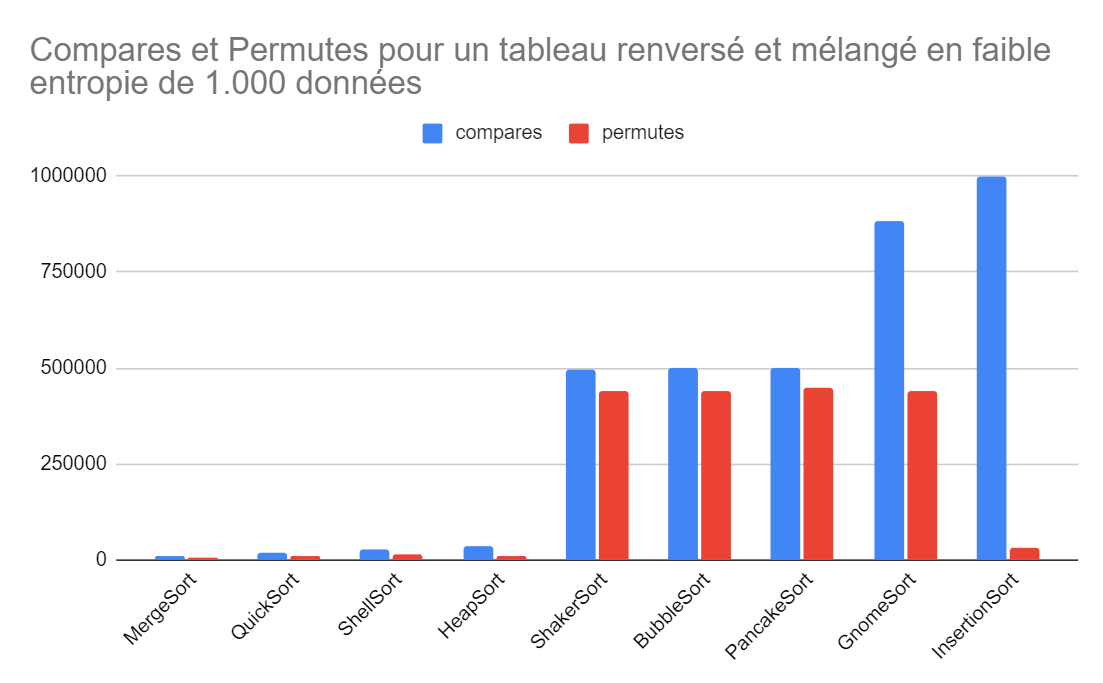
\includegraphics[scale=0.4]{Annexes/GrapheComparePermuteAllReverseFaible.PNG}
\newline
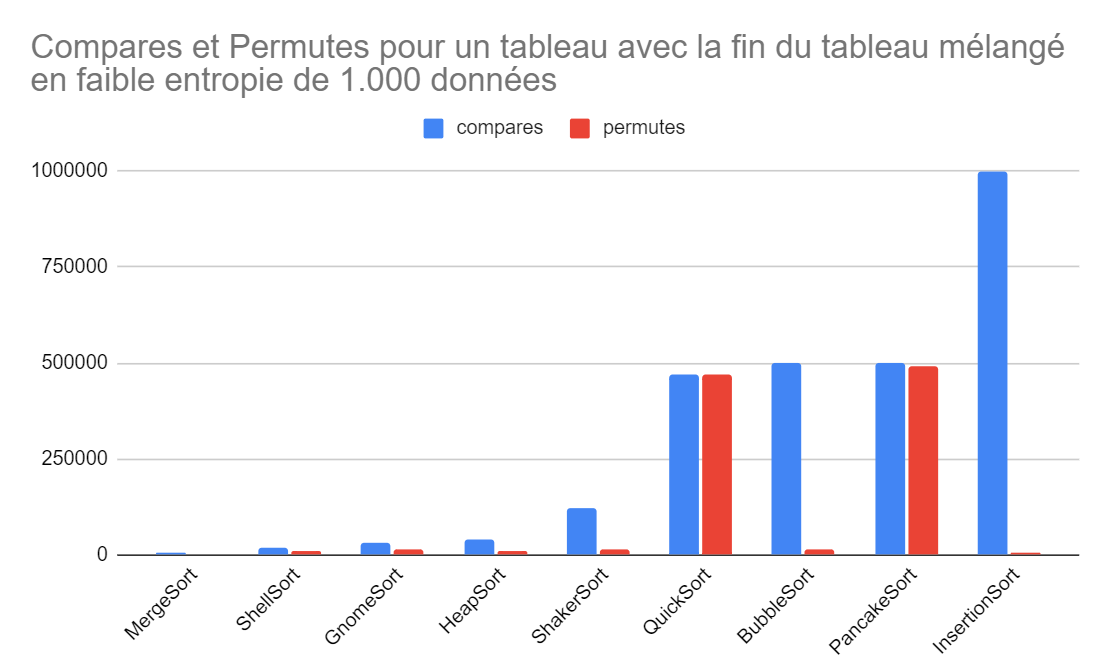
\includegraphics[scale=0.4]{Annexes/GrapheComparePermuteAllShuffleTail.PNG}
\newline
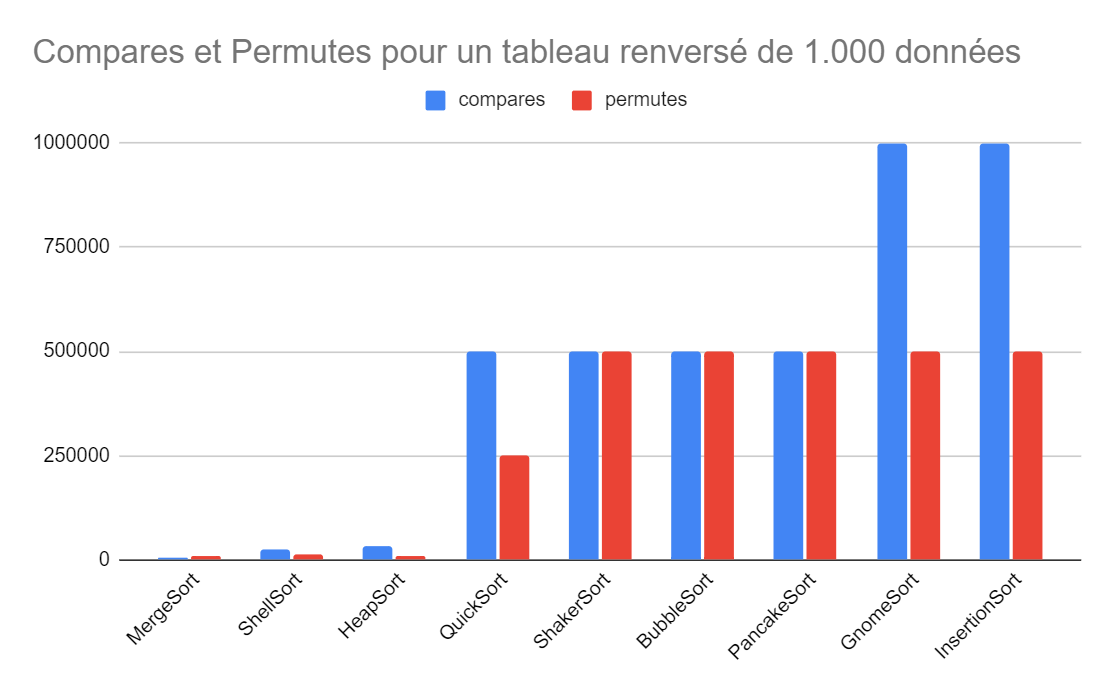
\includegraphics[scale=0.4]{Annexes/GrapheComparePermuteAllReverseTab.PNG}

\subsection{Analyse des résultats}
Dans le cas 1, voit une forte distinction entre nos algorithmes nlogn et nos algorithmes en n**2. Aucune surprise ici.
\newline
\newline
Dans le cas 2 on remarque que les algorithmes en nlogn ne changent pas beaucoup, cependant le GnomeSort et le ShakerSort savent efficacement trier le tableau, presque aussi efficacement que nos algos en nlogn
\newline
\newline
Dans le cas 3 on a des résultats similaires que dans le cas 1, mais avec la différence notable que les permutation et les comparaisons sont beaucoup plus proches. Ceci est attendu, avec un tableau inversé presque chaque comparaison devra donner lieu à une permutation
\newline
\newline
Dans le cas 3 il n'y a pas beaucoup de remarquable, les résultats sont similaires. Il est quand même très important de noter que QuickSort est très lent à faire le tri, et se retrouve a faire autant d'opérations que les tris en n**2

\section{Conclusion}
Chaque tri à des spécificités. Certains tris sont stables au niveau du nombre d'opérations, comme le mergesort et le bubble sort, alors que d'autres tris sont très efficaces dans certains cas spécifiques, mais souvent cette grande efficacité vient au coût d'une très grande inefficacité dans d'autres cas, comme le quicksort extrêmement lent à trier un tableau dont la fin est triée.\newline
Dans le cas général, l'utilisation du mergesort semble être sur, mais avec certaines informations sur la répartition de nos données, il peut être utile de connaitre d'autres tris qui peuvent être parfait pour nos besoins.\newline
Il y a bien sur les tris plus ludiques comme le bogosort, que nous avons choisis de ne pas analyser afin d'obtenir des résultats avant la fin de l'univers

\subsection{Récapitulatif de la problématique et de la réalisation}
Notre but était de comparer des algorithmes de tri pour voir comment le désordre influait sur le fonctionnement de ceux-ci. Nous avons donc créé un générateur et des algorithmes de tri à tester.

\subsection{Propositions d'améliorations}
En guise d'améliorations nous avons plusieurs propositions : 
\begin{itemize}
    \item Une interface de démarrage d'algorithme où nous pouvons choisir l'algorithme, le type de mélange, l'entropie et la taille du tableau.  \item Nous pourrions toujours rajouter des algorithmes de tri, nous en avons implémenté qu'une partie parmi tout ceux existants
    \item Dans l'idéal nous aurions pu essayer de créer notre propre algorithme de tri, même si c'est un projet très ambitieux.
\end{itemize}
\section{Problèmes rencontrées}
\subsection{Traitement des données}
Lors du développement de notre projet, nous avons réussi très rapidement à implémenter de nombreux algorithmes de tri ainsi qu'une visualisation de leur tri en action.\newline
Malheureusement pour la partie analyse de leur efficacité nous avons eu de nombreuses approches qui n'ont pas fonctionné.\newline
Dans un premier temps notre idée était de stocker les résultats dans un fichier sous format json, afin de pouvoir facilement lire, éditer et réécrire les données. Nous n'avons pas pu trouver de librairie qui permettait toute ces fonctionnalités, donc nous avons essayé de créé notre propre librairie à base d'ANTLR et les principes vu dans notre cours de Théorie des Langages et Compilation. Nous avons abandonnées cette approche  avoir rencontré des problèmes au niveau de l'intégration de notre librarie dans le projet.\newline
Finalement, par manque de temps, nous avons implémentees une approche rudimentaire sous format txt.
\subsection{Radix}
Le tri radix n'étant pas un tri par comparaison comme les autres tris, c'était difficile de choisir une métrique juste que l'on pouvait utiliser pour le comparer avec les autres.\newline
De plus, le fait qu'il n'était pas par comparaison à fait que nous n'avons pas réussi à en faire une visualisation
\end{document}
